%!TEX encoding = UTF-8 Unicode
%!TEX root = ../lect-w08.tex

\Subsection{Integrerad utvecklingsmiljö (IDE)}

\begin{Slide}{Välja IDE}\SlideFontSmall
\begin{itemize}
\item En \Emph{integrerad utvecklingsmiljö} \Eng{Integrated Development Environment, IDE} innehåller \\ editor + kompilator + debugger + en massa annat\\och gör utvecklingen enklare när man lärt sig alla finesser.

\item Läs om vad en IDE kan göra i appendix.

\pause

\item På LTH:s datorer finns två populära IDE installerade:
\begin{enumerate}\SlideFontSmall

\item \Emph{IntelliJ IDEA} (välj installera Scala-plugin när du kör första gången)
\begin{REPL}[numbers=none]
> idea
\end{REPL}

\item \Emph{Eclipse} med plugin \Emph{ScalaIDE} förinstallerad
\begin{REPL}[numbers=none]
> scalaide
\end{REPL}

\end{enumerate}
Läs mer om dessa i appendix innan du väljer vilken du vill lära dig.
\\Där står även hur du installerar dem på din egen dator.
\\IntelliJ anses av många för tillfället ha det bästa Scala-stödet, men är du van vid Eclipse så kan du lika gärna välja ScalaIDE.
\end{itemize}
\end{Slide}

\begin{Slide}{IntelliJ IDEA med Scala-plugin}
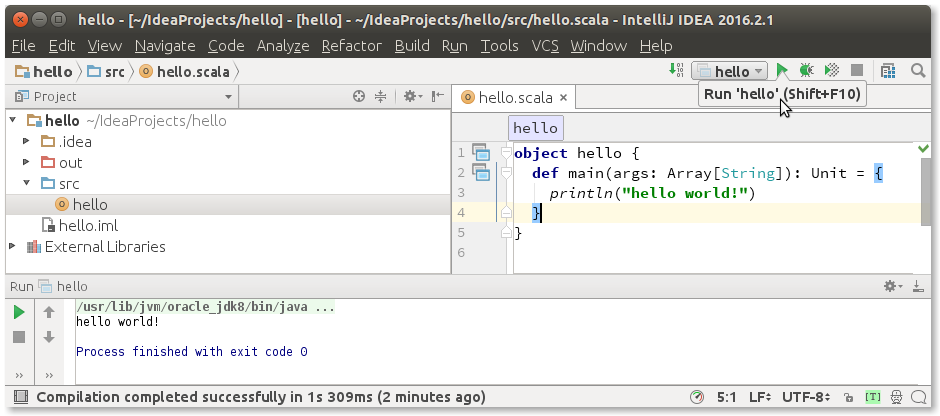
\includegraphics[width=\textwidth]{../img/intellij/idea-hello.png}
\end{Slide}

\begin{Slide}{Eclipse med ScalaIDE}
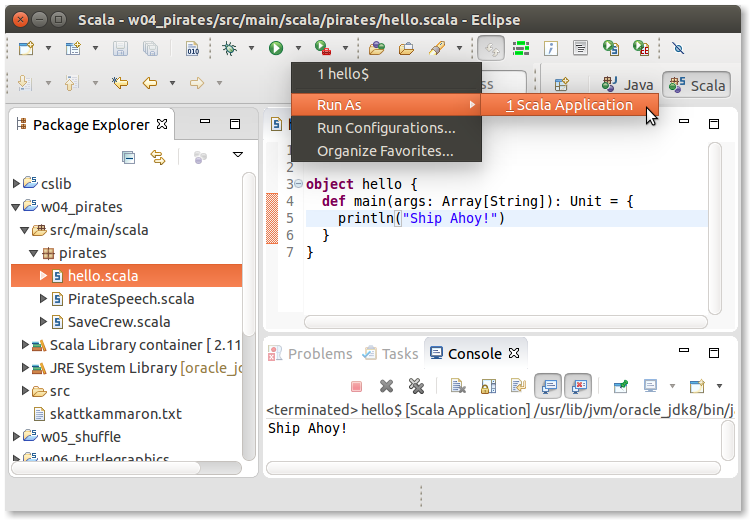
\includegraphics[width=\textwidth]{../img/eclipse/eclipse-pirates-hello.png}
\end{Slide}
